\documentclass[12pt]{article}
\usepackage{graphicx}
\title{CSIS 200: Software Tools for Physicists Final Project}

\begin{document}

\begin{abstract}

	This paper details the methods used to compute solutions to different probability
	based problems all having to do with the weather. The problems either ask about the 
	amount of days it rains in a month (one month is 30 days for simplicity), or about the 
	amount it rains, 
	or both. Some of the problems are solved analytically (like on pen and paper), and all of 
	the problems are solved numerically (generating numbers to use as fake data in order 
	to solve the problem). In the first problem, the probability of rain is 20\%, and it asks for 
	the probability it rains only one day in any given month. This is computed both 
	analytically and numerically, and the probability is 0.928\%. In the second problem, the 
	probability of rain is 10\% and the probability it rains at least eight days in a month is 
	around 08\%. In the third problem, the probability of rain depends on whether or not
	it rained the day before and, if it rains, the amount of rain has different probabilities. 
	The probability it rains at least 10~cm in any given month is 40\% and the average
	rainfall is 8.9 cm. A histogram was plotted for this problem and the uncertainty was
	calculated as well.

\end{abstract}
\section{Introduction}

	This final project is cumulative of everything taught in the course CSIS 200: 
	Software Tools for Physicists. It tests how much students truly learned in the
	course by requiring them to pull together all the coding skills taught throughout the 
	semester into one functional code for every problem. Although most of the 
	assigned problems can be worked out by hand analytically, students only receive 
	credit for solving them numerically in Jupyter Notebook. Solving a problem numerically
	is when data is gathered/produced and tested, and the conclusions of the data tests
	are the answers. By using the numerical method, students must use everything they 
	have learned from the beginning of the course all the way to the end of the course. This 
	includes everything from variables to loops and functions, and all the way to the 
	numpy.random.random function. If a student can successfully use all the tools they 
	have learned in the course to solve the problems given, then they have truly learned the 
	course material.

\section{Problem 1}

	In the first problem, the odds of it raining on any given day in a month is 20\%, and
	for simplicity, one month is thirty days. The question asked is: what are the odds of it 
	raining only one day out of the month?
	
	\subsection{Analytic Approach}
	
	The probability of it raining on any given day is 20\%, or 0.2. This means the probability
	of it not raining on any given day is 80\%, or 0.8. To find the probability of it raining only 
	once in one month, the probability of it raining only once and not raining the other 29
	days must be calculated. In probability, ``and'' means multiply. Also, because the one 
	day of rain could occur on any of the days of the month, the probabilities must be 
	multiplied by 30. So the equation should look like this: 
	
	$$P = ((P_{rain}) * (P_{dry})^{29} * 30* 100\%$$
	
	$$P = \frac{1}{5} * (\frac{4}{5})^{29} * 30 * 100\%$$
	
	$$P = 0.928\%$$
	
	The analytical approach results in the conclusion that the probability of it raining only 
	one day of the month is 0.928\%.
	
	\subsection{Numerical Approach}
	
	To solve this problem numerically, first a function
	that takes in a list of thirty random numbers between one and five was defined (where 
	one is a day it rains and 2 through 5 are days it does not rain).  A variable was set
	equal to zero to track the number of days it rained and another variable was set equal 
	to False. Then the function loops over the the list of thirty numbers and, using an if 
	statement, if one of the numbers in the list is equal to one, then it adds one to the 
	variable tracking the number of days it rains. After the function loops over the list, 
	outside of the for-loop it looks at whether or not the variable 
	tracking the number of rainy days is equal to one. If it is equal to one, the other variable 
	becomes True. The function returns the variable that will either be True or False.
	
	Next, a Monte Carlo approach is used to test numerically the probability of rain by 
	generating fake data. A variable is set equal to the number of months tested. Note that
	the higher this
	number is, the more accurate the answer is, but the longer it takes to compute the 
	answer. Another variable is set to zero to track the number of months it rains only one 
	day. A list from zero to the number of months tested is then looped over, and for every 
	month, a list of thirty 	numbers between one and five is generated using the 
	numpy.random.randint function. Calling the function and using an if 
	statement, if a month has one day of rain only, the variable tracking the number 
	of months increases by one. Dividing this by the total number of months and multiplying
	 by one hundred consistently gives an answer around 0.9\%, which close to the 
	analytical answer, but not exactly. The answer is different every time the program is run 
	because it generates different numbers between one and five every time.

\section{Problem 2}

	Problem 2 states there is a 10\% chance that it will rain on any given day in a month
	 and asks the probability that it rains at least eight days in any order in a month.
	 
	Like in Problem 1, a function that takes in a list of thirty random numbers between one 
	and five was defined, a variable was set equal to zero to track the rainy days, and
	another variable was set equal to False. The function loops over a list of thirty random 
	numbers between one and ten (because the probability of rain is now 10\%) and every
	time one of the numbers in the list is one, the variable set equal to zero increases by
	 one. After the function loops over the list, it looks at the  
	variable tracking the rainy days and if it is greater than or equal to eight, the other 
	variable originally set to False becomes True. The function returns this True/False
	variable.
	
	Then, like in Problem 1, a variable is set to the number of months to test and another 
	is set equal to zero this time to count the number of days it rains a least eight days.
	Then a list of all the months is looped over and for every month a list of thirty random 
	numbers between one and ten is generated using the numpy.random.randint function. 
	Then using an if statement and calling the function, if a month has greater than or equal 
	to eight days of rain, the variable tracking the number of months with at least eight days
	of rain increases by one. By dividing this by the total number of months and multiplying
	 by one hundred, and the answer is consistently around 0.8\%.


\section{Problem 3}

\subsection{Part A}

	This question asks for the probability it will rain at least 10~cm in any given month, 
	given the following conditions.
	
	The odds of it raining depend on if it rained the day before:
	\begin{itemize}
		\item If it is the first day of the month, there is a 10\% chance of rain
		\item If it rained one day before but not two days before, there is a 20\% 
		chance of rain
		\item If it rained both of the two days before, but not the third day before, there is a 
		25\% chance of rain 
		\item If it rained for three or more days before, then there is a 25\% chance of rain
		\item Otherwise there is a 10\% chance of rain. 
	\end{itemize}
	If it does, in fact, rain, then the probabilities of certain amounts of rainfall are:
	\begin{itemize}
		\item 20\% 1 cm of rain
		\item 30\% 2 cm of rain
		\item 30\% 3 cm of rain
		\item 10\% 4 cm of rain
		\item 5\% 5 cm of rain.
	\end{itemize}
	
	
	To solve this problem numerically, first a function was defined to keep track of when it
	does actually rain. The input to this function will be a list of thirty random numbers 
	between zero and one. In the function, first a variable was set equal to zero (in order to
	count the days it rains) and another variable was set equal to the length of the input.
	Then, using a for loop, the function loops over the the list from zero to the variable set 
	equal to the length of the list. This is so that the conditionals in the loop can look at the 
	values of the numbers (i.e. a number between zero and one) that come one, two, or 
	three days, or places, before the day the function is looking at. First the loop looks at
	the three days before. If 
	three days before is less than or equal to 0.1 and two days before is less than or equal 
	to 0.2 and the day before is less than or equal to 0.25 (which means it rained all three 
	days before this day), then if the number in the loop is less then or equal to 0.05, one is 
	added to the variable counting the amount of days it rained. Next, if the number in the 
	loops is not satisfied by that condition, the loop looks at 
	the three days before the day that the loop is on. If the second day before is 
	less than or equal to 0.1 and the day before is less than or equal to 0.2 (meaning it 
	rained both days before), but the third day before is greater than 0.1 (meaning it did not 
	rain the third day before, then if the number the loop is looking at is less than or equal 
	to 0.25, it means it rained that day and the variable tracking the amount of days it
	rained increases by one. Then, if the number does not meet those conditions, the loop
	looks at the day before and if the value of the day before is less than or equal to 0.1 
	(meaning it rained the day before), and if two days before the valued is greater than 0.1 
	(meaning it didn't rain two days before), then if the value of the number in the loop is 
	less than or equal to 0.2, then the function adds one to the variable counting the days it 
	rained. Lastly, if none of those conditions are met, then if the number in the loop is less
	than or equal to 0.1, it rained that day and the variable tracking the days it rained 
	increases by one. This process is repeated for every number in the loop and the 
	function returns the variable tracking the number of days in the loop.
	
	
	Next, a function to track how much it rained was defined. The input to this function will 
	be the output of the first function. First, a random list of numbers between zero and
	one is generated and the length of the list depends on the input of the function. So 
	every day it rained has a random value from zero to one assigned to it. A 
	variable is set to zero to count the centimeters of rainfall for each day it rains. The 
	function loops over the list generated and if it is less than or equal to 0.2, the variable 
	tracking the rainfall, or the tracking variable, increases by one (cm). Else, if the number 
	is greater than 0.2 but less than or equal to 0.5, then the tracking variable increases by 
	two (cm). Else, if the number is greater than 0.5 but less than or equal to 0.8, then the 
	tracking variable increases by three (cm). Else, if the number is greater than 0.8 and 
	less than or equal to 0.9, then the tracking variable increases by four (cm). Lastly, if the 
	number is greater than 0.9 but less than or equal to 1.0, then five (cm) is added to the 
	tracking variable. The loop does this for every variable in the list. The function returns 
	the variable tracking the rainfall.
	
	Finally, many months can be tested. First, a variable is set to a number (the higher the 
	number, the more accurate the answer, but the longer the code takes to run) and 
	another variable is set equal to zero to track the amount of months with at least 10~cm 
	of rain. Then a for loop loops over the same amount of times as the first variable is set
	to. In the loop, so for every month, a variable is set equal to a list of thirty numbers 
	between zero and one. A second variable is set equal to the output of the first function
	that tracks if/when it rains with the input of the variable equal to the list of thirty random 
	numbers between zero and one. Then, for the output of the second function defined 
	with the input as the second variable (equal to how many days it rained), if it is greater 
	than or equal to ten, the variable tracking the number of months it rained 10~cm 
	increases by one. The number of months it rains at least 10~cm is divided by the total 
	number of months and multiplied by 100\%.  The answer is consistently around 40\%.
	

\subsection{Part B}

	Before making a histogram of the rainfall, the data from Part~A was put into an array by
	setting a variable equal to an empty array and looping over a list of the number of 
	test months. For every month, a list of 30 random numbers between zero and one was 
	created. This list was put through the function that tracked the number of rainy days,
	and then the output of that function was the input to the function that tracked how much 
	rain fell. The amount of rainfall was appended to the empty array. This repeated for 
	however many months were tested. Then the array of the amount of rainfall for each 
	month was plotted into a histogram. See Figure~\ref{histo} for a sample!
	
	\begin{figure}[h]
	
		\centering
		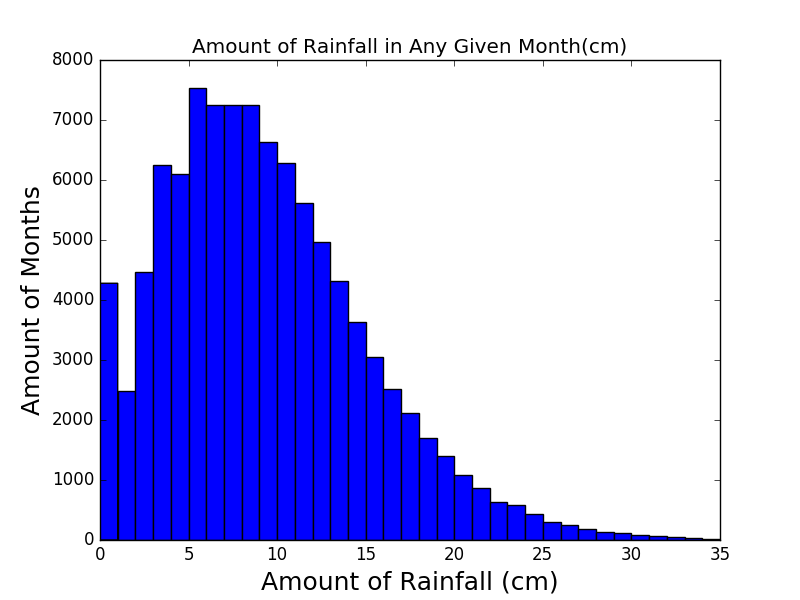
\includegraphics[width=.9\textwidth]{Rain_Histogram.png}
		\caption{This is a histogram for a test of 100,000 random months \label{histo}}
	
	\end{figure}

\subsection{Part C}

	To calculate the average rainfall in any given month, the function numpy.mean() was
	used. The input to this function is the array created in Part~B. The average amount of 
	rainfall in a month was consistently around 8.9 cm.

\subsection{Part D}

	To calculate the uncertainty, the middle 95\% of the data was found and the outside
	edges of the range (the lower 2.5\% and the higher 2.5\%) were used. There is 95\%
	confidence that the rainfall will be between 0 cm and 22 cm.


\end{document}